\subsubsection{UC10 - Gestione veicoli}
  \begin{figure}[H]
 	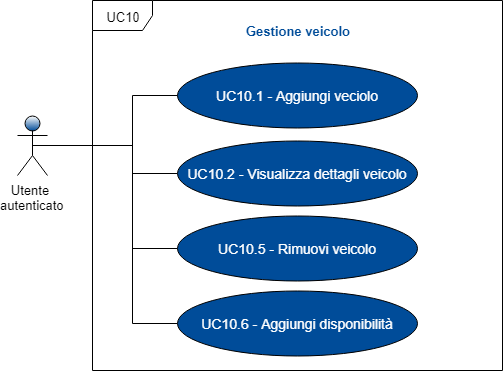
\includegraphics[width=10cm]{res/images/UC10Gestioneveicolo.png}
 	\centering
 	\caption{UC10 - Gestione veicoli}
 \end{figure}
 \begin{itemize}
 	\item \textbf{Attori Primari}: utente autenticato;
 	\item \textbf{Descrizione}: l'utente ha una panoramica dei veicoli che ha inserito visualizzando solo poche cose riguardanti il mezzo quali:
 	\begin{itemize}
 		\item marca del veicolo;
 		\item modello del veicolo;
 		\item immagine del veicolo;
 		\item anno d'immatricolazione.
 	\end{itemize} 
 	e ha la possibilità di aggiungere un veicolo o visualizzare i dettagli del veicolo;
 	\item \textbf{Scenario principale}: l'utente visualizza il parco macchine a disposizione e può decidere se:
 	\begin{itemize}
 		\item aggiungere un veicolo [UC10.1];
 		\item visualizzare i dettagli di un veicolo già aggiunto [UC10.2];
 		\item rimuovere un veicolo [UC10.5];
 		\item aggiungere una disponibilità al veicolo [UC10.6].
 	\end{itemize}
 	\item \textbf{Precondizione}: l'utente accede al fragment\glosp per la gestione dei veicoli;
 	\item \textbf{Postcondizione}: l'utente visualizza le informazioni relative ai propri veicoli, con le eventuali operazioni disponibili su ognuno di essi.
 \end{itemize}
 \subsubsection{UC10.1 - Aggiungi veicolo}
 \begin{itemize}
 	\item \textbf{Attori Primari}: utente autenticato;
 	\item \textbf{Descrizione}: l'utente può aggiungere un mezzo di trasporto al proprio parco macchine;
 	\item \textbf{Scenario principale}: l'utente aggiunge un veicolo compilando gli appositi campi obbligatori, ovvero:
 	\begin{itemize}
 		\item inserimento immagine veicolo [UC10.1.1];
 		\item inserimento marca veicolo [UC10.1.2];
 		\item inserimento modello veicolo [UC10.1.3];
 		\item inserimento anno d'immatricolazione veicolo [UC10.1.4];
 		\item inserimento posizione veicolo [UC10.1.5];
 		\item inserimento costo orario [UC10.1.6].
 	\end{itemize}
 	e successivamente salverà il nuovo veicolo confermando i campi appena inseriti;
 	\item \textbf{Precondizione}: l'utente ha inserito correttamente tutti i campi necessari;
 	\item \textbf{Postcondizione}: il nuovo veicolo viene aggiunto ai veicoli posseduti.
 \end{itemize}
\begin{figure}[H]
	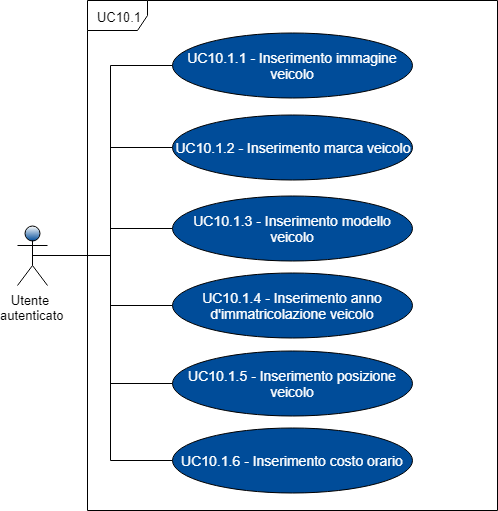
\includegraphics[width=10cm]{res/images/UC10-1Aggiungiveicolo.png}
	\centering
	\caption{UC10.1 - Aggiungi veicolo}
\end{figure}
\subsubsection{UC10.1.1 - Inserimento immagine veicolo}
\begin{itemize}
	\item \textbf{Attori Primari}: utente autenticato;
	\item \textbf{Descrizione}: al fine di portare a termine il processo di inserimento di un nuovo veicolo l'utente deve inserire un'immagine del proprio mezzo, campo ritenuto obbligatorio; 
	\item \textbf{Scenario principale}: l'utente preme il pulsante relativo all'inserimento dell'immagine del veicolo;	
	\item \textbf{Precondizione}: l'applicazione ha reso disponibile il bottone per l'inserimento dell'immagine del veicolo;
	\item \textbf{Postcondizione}: l'utente ha inserito correttamente l'immagine del veicolo.
\end{itemize}
\subsubsection{UC10.1.2 - Inserimento marca veicolo}
\begin{itemize}
	\item \textbf{Attori Primari}: utente autenticato;
	\item \textbf{Descrizione}: al fine di portare a termine il processo di inserimento di un nuovo veicolo l'utente deve inserire la marca, campo ritenuto obbligatorio;
	\item \textbf{Scenario principale}: l'utente compila il campo relativo alla marca del veicolo;	
	\item \textbf{Precondizione}: l'applicazione ha reso disponibile il campo per l'inserimento della marca del veicolo;
	\item \textbf{Postcondizione}: l'utente ha compilato il campo con la marca.	
\end{itemize}
\subsubsection{UC10.1.3 - Inserimento modello veicolo}
\begin{itemize}
	\item \textbf{Attori Primari}: utente autenticato;
	\item \textbf{Descrizione}: al fine di portare a termine il processo di inserimento di un nuovo veicolo l'utente deve inserire il modello, campo ritenuto obbligatorio;
	\item \textbf{Scenario principale}: l'utente compila il campo relativo alla marca del veicolo;	
	\item \textbf{Precondizione}: l'applicazione ha reso disponibile il campo per l'inserimento il modello del veicolo;
	\item \textbf{Postcondizione}: l'utente ha compilato il campo con il modello.	
\end{itemize}
\subsubsection{UC10.1.4 - Inserimento anno d'immatricolazione veicolo}
\begin{itemize}
	\item \textbf{Attori Primari}: utente autenticato;
	\item \textbf{Descrizione}: al fine di portare a termine il processo di inserimento di un nuovo veicolo l'utente deve inserire l'anno di immatricolazione, campo ritenuto obbligatorio;
	\item \textbf{Scenario principale}: l'utente compila il campo relativo all'anno d'immatricolazione del veicolo;	
	\item \textbf{Precondizione}: l'applicazione ha reso disponibile il campo per l'inserimento dell'anno d'immatricolazione del veicolo;
	\item \textbf{Postcondizione}: l'utente ha compilato il campo con l'anno d'immatricolazione.	
\end{itemize}
\subsubsection{UC10.1.5 - Inserimento posizione veicolo}
\begin{itemize}
	\item \textbf{Attori Primari}: utente autenticato;
	\item \textbf{Descrizione}: al fine di portare a termine il processo di inserimento di un nuovo veicolo l'utente deve inserire la posizione del proprio mezzo, campo ritenuto obbligatorio;
	\item \textbf{Scenario principale}: l'utente compila il campo relativo alla posizione del veicolo;	
	\item \textbf{Precondizione}: l'applicazione ha reso disponibile il campo per l'inserimento della posizione del veicolo;
	\item \textbf{Postcondizione}: l'utente ha compilato il campo con la posizione del veicolo.	
\end{itemize}
\subsubsection{UC10.1.6 - Inserimento costo orario}
\begin{itemize}
	\item \textbf{Attori Primari}: utente autenticato;
	\item \textbf{Descrizione}: al fine di portare a termine il processo di inserimento di un nuovo veicolo l'utente deve inserire il costo orario in euro del proprio mezzo, campo ritenuto obbligatorio;
	\item \textbf{Scenario principale}: l'utente compila il campo relativo al costo orario in euro;	
	\item \textbf{Precondizione}: l'applicazione ha reso disponibile il campo per l'inserimento del costo orario in euro;
	\item \textbf{Postcondizione}: l'utente ha compilato il campo con il costo orario in euro.	
\end{itemize}
\subsubsection{UC10.2 - Visualizza dettagli veicolo}
\begin{itemize}
	\item \textbf{Attori Primari}: utente autenticato;
	\item \textbf{Descrizione}: l'utente autenticato, per ogni veicolo, può visualizzare in dettaglio le seguenti informazioni:
	\begin{itemize}
		\item marca;
		\item modello;
		\item anno di immatricolazione;
		\item costo orario;
		\item rating.
	\end{itemize}
	e ha la possibilità di:
	\begin{itemize}
		\item visualizzare le disponibilità del veicolo [UC10.3];
		\item visualizzare le statistiche del veicolo[UC10.4];
		\item rimuoverlo [UC10.5].
	\end{itemize}
	\item \textbf{Scenario principale}: l'utente visualizza i dati di dettaglio del veicolo;
	\item \textbf{Precondizione}: l'utente autenticato visualizza i dettagli del veicolo;
	\item \textbf{Postcondizione}: l'utente autenticato ha visualizzato i dettagli del veicolo.
\end{itemize}
\begin{figure}[H]
	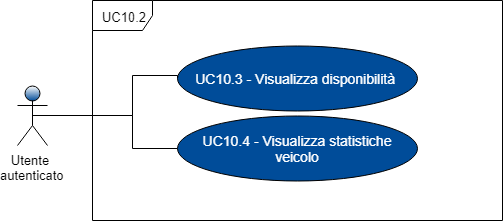
\includegraphics[width=10cm]{res/images/UC11Dettagli.png}
	\centering
	\caption{UC10.2 - Visualizza dettagli veicolo}
\end{figure}
\subsubsection{UC10.3 - Visualizza disponibilità}
\begin{itemize}
	\item \textbf{Attori Primari}: utente autenticato;
	\item \textbf{Descrizione}: l'utente ha una panoramica delle disponibilità fino ad ora aggiunte, per ognuna di queste viene visualizzata:
	\begin{itemize}
		\item la data;
		\item la fascia oraria;
	\end{itemize} 
	e ha la possibilità di aggiungere una disponibilità [UC10.6];
	\item \textbf{Scenario principale}: l'utente visualizza le disponibilità da lui aggiunte e può inserirne delle altre attraverso l'apposito pulsante;
	\item \textbf{Precondizione}: l'utente entra nella visualizzazione delle disponibilità del veicolo selezionato;
	\item \textbf{Postcondizione}: l'utente visualizza tutte le disponibilità del veicolo inserite. 
\end{itemize}
\subsubsection{UC10.4 - Visualizza statistiche}
\begin{itemize}
	\item \textbf{Attori Primari}: utente autenticato;
	\item \textbf{Descrizione}: l'utente ha una panoramica delle statistiche del proprio veicolo con grafici o dati che rappresentano come e quanto viene utilizzato un suo mezzo rispetto ad un altro e poter scegliere se tenere o aggiungere il veicolo. Si visualizzano i seguenti valori:
	\begin{itemize}
		\item frequenza giorni della settimana di utilizzo del veicolo;
		\item guadagno per giorni della settimana del veicolo;
		\item guadagno totale.
	\end{itemize}
	\item \textbf{Scenario principale}: l'utente visualizza le statistiche del proprio veicolo risultanti dalle varie prenotazioni effettuate;
	\item \textbf{Precondizione}: l'utente entra nella visualizzazione delle statistiche del veicolo selezionato;
	\item \textbf{Postcondizione}: l'utente visualizza l'andamento delle statistiche del veicolo. 
\end{itemize}
\subsubsection{UC10.5 - Rimuovi veicolo}
\begin{itemize}
	\item \textbf{Attori Primari}: utente autenticato;
	\item \textbf{Descrizione}: l'utente può rimuovere un mezzo di trasporto dal proprio parco macchine;
	\item \textbf{Scenario principale}: l'utente, dopo aver selezionato il veicolo da visualizzare, può rimuoverlo dal proprio parco macchine attraverso l'apposito pulsante;
	\item \textbf{Precondizione}: l'applicazione mostra all'utente i propri veicoli e ne permette la selezione;
	\item \textbf{Postcondizione}: il veicolo selezionato viene rimosso dal parco macchine.
\end{itemize}
\subsubsection{UC10.6 - Aggiungi disponibilità}
\begin{figure}[H]
	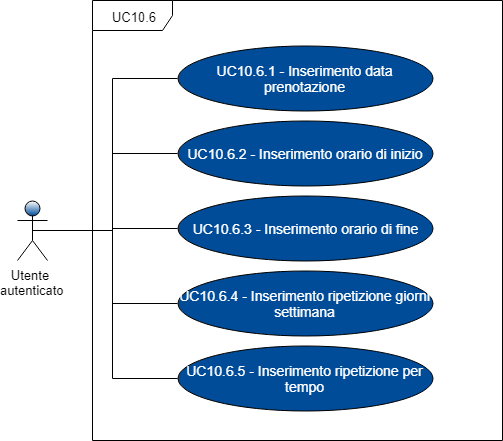
\includegraphics[width=11cm]{res/images/UC11Aggiungi.png}
	\centering
	\caption{UC10.6 - Aggiungi disponibilità}
\end{figure}
\begin{itemize}
	\item \textbf{Attori Primari}: utente autenticato;
	\item \textbf{Descrizione}: l'utente può inserire la disponibilità in cui mette a disposizione il proprio veicolo inserendo data, ora ed eventuale ripetizione delle stesse in giorni differenti;
	\item \textbf{Scenario principale}: l'utente, dopo aver visualizzato la lista delle disponibilità di un suo veicolo, decide di aggiungere un ulteriore disponibilità e viene portato nella sezione "singola" inserendo:
	\begin{itemize}
		\item data prenotazione [UC10.6.1];
		\item ora di inizio [UC10.6.2];
		\item ora di fine [UC10.6.3].
	\end{itemize}
	e successivamente confermando l'aggiunta della disponibilità, l'utente viene rimandato nell'area di \textit{Gestione veicolo};
	\item \textbf{Scenario alternativo}: l'utente, dopo aver visualizzato la lista delle disponibilità di un suo veicolo, decide di aggiungere un ulteriore disponibilità, cambia sezione ed entra in "ripetuta" inserendo:
	\begin{itemize}
		\item ora di inizio [10.6.2];
		\item ora di fine [10.6.3];
		\item ripetizione giorni settimana [10.6.4];
		\item ripetizione per quanto tempo [10.6.5].
	\end{itemize}
	e successivamente confermando l'aggiunta della disponibilità, l'utente viene rimandato nell'area di \textit{Gestione veicolo};
	\item \textbf{Precondizione}: l'applicazione mostra all'utente la lista delle disponibilità fino ad ora aggiunte e ne permette ulteriore inserimento;
	\item \textbf{Postcondizione}: viene aggiunta la disponibilità al veicolo selezionato.
\end{itemize}
\subsubsection{UC10.6.1 - Inserimento data prenotazione}
\begin{itemize}
	\item \textbf{Attori Primari}: utente autenticato;
	\item \textbf{Descrizione}: al fine di portare a termine il processo di aggiunta della disponibilità al veicolo, l'utente deve inserire la data di prenotazione. Visualizzerà un calendario dove potrà selezionare un giorno del mese che preferisce;
	\item \textbf{Scenario principale}: l'utente compila il campo relativo alla data di prenotazione;	
	\item \textbf{Precondizione}: l'applicazione ha reso disponibile il campo per l'inserimento della data di prenotazione;
	\item \textbf{Postcondizione}: l'utente ha compilato il campo con la data di prenotazione.	
\end{itemize}
\subsubsection{UC10.6.2 - Inserimento ora di inizio}
\begin{itemize}
	\item \textbf{Attori Primari}: utente autenticato;
	\item \textbf{Descrizione}: al fine di portare a termine il processo di aggiunta della disponibilità al veicolo, l'utente deve inserire l'ora di inizio in cui un usufruente può prenotare l'auto. L'orario viene mostrato in fasce orarie da 15 minuti;
	\item \textbf{Scenario principale}: l'utente compila il campo relativo all'ora di inizio;	
	\item \textbf{Precondizione}: l'applicazione ha reso disponibile il campo per l'inserimento dell'ora di inizio;
	\item \textbf{Postcondizione}: l'utente ha compilato il campo con l'ora di inizio.	
\end{itemize}
\subsubsection{UC10.6.3 - Inserimento ora di fine}
\begin{itemize}
	\item \textbf{Attori Primari}: utente autenticato;
	\item \textbf{Descrizione}: al fine di portare a termine il processo di aggiunta della disponibilità al veicolo, l'utente deve inserire l'ora di fine in cui un usufruente può prenotare l'auto. L'orario viene mostrato in fasce orarie da 15 minuti;
	\item \textbf{Scenario principale}: l'utente compila il campo relativo all'ora di fine;	
	\item \textbf{Precondizione}: l'applicazione ha reso disponibile il campo per l'inserimento dell'ora di fine;
	\item \textbf{Postcondizione}: l'utente ha compilato il campo con l'ora di fine.	
\end{itemize}
\subsubsection{UC10.6.4 - Inserimento ripetizione giorni della settimana}
\begin{itemize}
	\item \textbf{Attori Primari}: utente autenticato;
	\item \textbf{Descrizione}: al fine di portare a termine il processo di aggiunta della disponibilità al veicolo, l'utente deve inserire i giorni della settimana in cui vuole che il veicolo sia disponibile;
	\item \textbf{Scenario principale}: l'utente compila il campo relativo all'inserimento dei giorni della settimana in cui ripetere la disponibilità;	
	\item \textbf{Precondizione}: l'applicazione ha reso disponibile il campo per l'inserimento dei giorni della settimana in cui rendere disponibile il veicolo;
	\item \textbf{Postcondizione}: l'utente ha compilato il campo con i giorni della settimana in cui vuole ripetere la disponibilità.	
\end{itemize}
\subsubsection{UC10.6.5 - Inserimento ripetizione per tempo}
\begin{itemize}
	\item \textbf{Attori Primari}: utente autenticato;
	\item \textbf{Descrizione}: al fine di portare a termine il processo di aggiunta della disponibilità al veicolo, l'utente deve inserire la quantità di tempo in cui la disponibilità del veicolo deve essere ripetuta (per esempio: una settimana, due settimane, un mese, etc);
	\item \textbf{Scenario principale}: l'utente compila il campo relativo all'inserimento della quantità di tempo in cui la disponibilità del veicolo deve essere ripetuta;	
	\item \textbf{Precondizione}: l'applicazione ha reso disponibile il campo per l'inserimento della quantità di tempo in cui la disponibilità del veicolo deve essere ripetuta;
	\item \textbf{Postcondizione}: l'utente ha compilato il campo con la quantità di tempo in cui la disponibilità del veicolo deve essere ripetuta.	
\end{itemize}